\documentclass[a4paper,14pt]{extarticle}

\usepackage[a4paper,margin=2.5cm]{geometry}
\usepackage{iftex}
\ifPDFTeX
  \usepackage[T2A]{fontenc}
  \usepackage[utf8]{inputenc}
  \usepackage[russian]{babel}
  \usepackage{tempora}
\else
  \usepackage[russian]{babel}
  \usepackage{fontspec}
  \setmainfont{Times New Roman}
\fi

\usepackage{amsmath}
\usepackage{amssymb}
\usepackage{graphicx}
\usepackage{float}
\usepackage{booktabs}
\usepackage{setspace}
\usepackage{xcolor}
\usepackage{listings}
\usepackage{fancyvrb}
\usepackage{subcaption}

\onehalfspacing

\lstdefinestyle{pycode}{
    language=Python,
    basicstyle=\ttfamily\small,
    keywordstyle=\color{blue!70!black},
    commentstyle=\color{green!40!black},
    stringstyle=\color{orange!60!black},
    showstringspaces=false,
    breaklines=true,
    frame=single,
    tabsize=4
}

\begin{document}

% Титульный лист
\begin{titlepage}
    \centering

    \IfFileExists{fefu.jpg}{
        
\includegraphics[scale=0.15]{fefu.jpg}\\[0.4cm]
    }{
        \vspace*{1.8cm}
    }

    МИНИСТЕРСТВО НАУКИ И ВЫСШЕГО ОБРАЗОВАНИЯ\\
    РОССИЙСКОЙ ФЕДЕРАЦИИ\\
    Федеральное государственное автономное образовательное учреждение высшего образования\\
    \textbf{«Дальневосточный федеральный университет»}\\
    \textbf{(ДВФУ)}\\[0.3cm]
    \rule{\linewidth}{0.7mm}\\[0.3cm]

    \textbf{ИНСТИТУТ МАТЕМАТИКИ И КОМПЬЮТЕРНЫХ ТЕХНОЛОГИЙ}\\[0.3cm]
    \textbf{Кафедра математического и компьютерного моделирования}\\[0.9cm]

    Захватов Дмитрий Алексеевич\\
    \textbf{ЛАБОРАТОРНАЯ РАБОТА №1: ВЫБОРКА}\\[0.3cm]

    Направление подготовки 02.03.01 СЦТ «Сквозные цифровые технологии»,\\
    образовательная программа «Математика и компьютерные науки»,\\
    очная форма обучения\\[1cm]

    \raggedleft
    \textbf{Студент группы Б9123-02.03.01сцт2}\\
    \rule{4.5cm}{0.3mm} Д.\,А.~Захватов\\[1cm]

    \textbf{Руководитель проекта}\\
    \rule{4.2cm}{0.3mm} К.\,А.~Ганжа

    \vfill
    \centering
    Владивосток\\
    2026
\end{titlepage}

\section*{2. Краткое математическое описание методов и синтаксис в Python}

В работе сформированы 8 выборок из 4 распределений (по 2 объема: 100 и 1000) и вычислены:
\[
\bar{x}=\frac{1}{n}\sum_{i=1}^{n}x_i,\qquad
D=\frac{1}{n}\sum_{i=1}^{n}(x_i-\bar{x})^2,\qquad
s=\sqrt{D}.
\]

\textbf{Равномерное распределение:} \(X\sim U(a,b)\), где \(a=2\), \(b=7\).\\
Синтаксис:
\begin{lstlisting}[style=pycode]
st.uniform.rvs(loc=2, scale=5, size=100, random_state=16)
st.uniform.rvs(loc=2, scale=5, size=1000, random_state=16)
\end{lstlisting}

\textbf{Распределение Бернулли:} \(X\sim B(p)\), где \(p=0.27\).\\
Синтаксис:
\begin{lstlisting}[style=pycode]
st.bernoulli.rvs(p=0.27, size=100, random_state=16)
st.bernoulli.rvs(p=0.27, size=1000, random_state=16)
\end{lstlisting}

\textbf{Биномиальное распределение:} \(X\sim Bin(n,p)\), где \(n=12\), \(p=0.35\).\\
Синтаксис:
\begin{lstlisting}[style=pycode]
st.binom.rvs(n=12, p=0.35, size=100, random_state=16)
st.binom.rvs(n=12, p=0.35, size=1000, random_state=16)
\end{lstlisting}

\textbf{Нормальное распределение:} \(X\sim N(\mu,\sigma^2)\), где \(\mu=4.5\), \(\sigma=1.8\).\\
Синтаксис:
\begin{lstlisting}[style=pycode]
st.norm.rvs(loc=4.5, scale=1.8, size=100, random_state=16)
st.norm.rvs(loc=4.5, scale=1.8, size=1000, random_state=16)
\end{lstlisting}

\section*{3. Результаты}

\subsection*{3.1 Таблица результатов}
\begin{table}[H]
\centering
\caption{Сравнение выборочных характеристик (свои функции и numpy)}
\small
\begin{tabular}{rcccccc}
\toprule
№ & Среднее\_свое & Дисперсия\_своя & Std\_свое & Среднее\_numpy & Дисперсия\_numpy & Std\_numpy \\
\midrule
1 & 4.482376 & 2.094645 & 1.447289 & 4.482376 & 2.094645 & 1.447289 \\
2 & 4.450935 & 2.085030 & 1.443963 & 4.450935 & 2.085030 & 1.443963 \\
3 & 0.250000 & 0.187500 & 0.433013 & 0.250000 & 0.187500 & 0.433013 \\
4 & 0.250000 & 0.187500 & 0.433013 & 0.250000 & 0.187500 & 0.433013 \\
5 & 4.190000 & 2.493900 & 1.579209 & 4.190000 & 2.493900 & 1.579209 \\
6 & 4.134000 & 2.740044 & 1.655308 & 4.134000 & 2.740044 & 1.655308 \\
7 & 4.537930 & 3.154746 & 1.776160 & 4.537930 & 3.154746 & 1.776160 \\
8 & 4.462000 & 3.174096 & 1.781599 & 4.462000 & 3.174096 & 1.781599 \\
\bottomrule
\end{tabular}
\end{table}


\subsection*{3.2 Графики (8 шт.)}

\begin{figure}[H]
    \centering
    \begin{subfigure}{0.48\textwidth}
        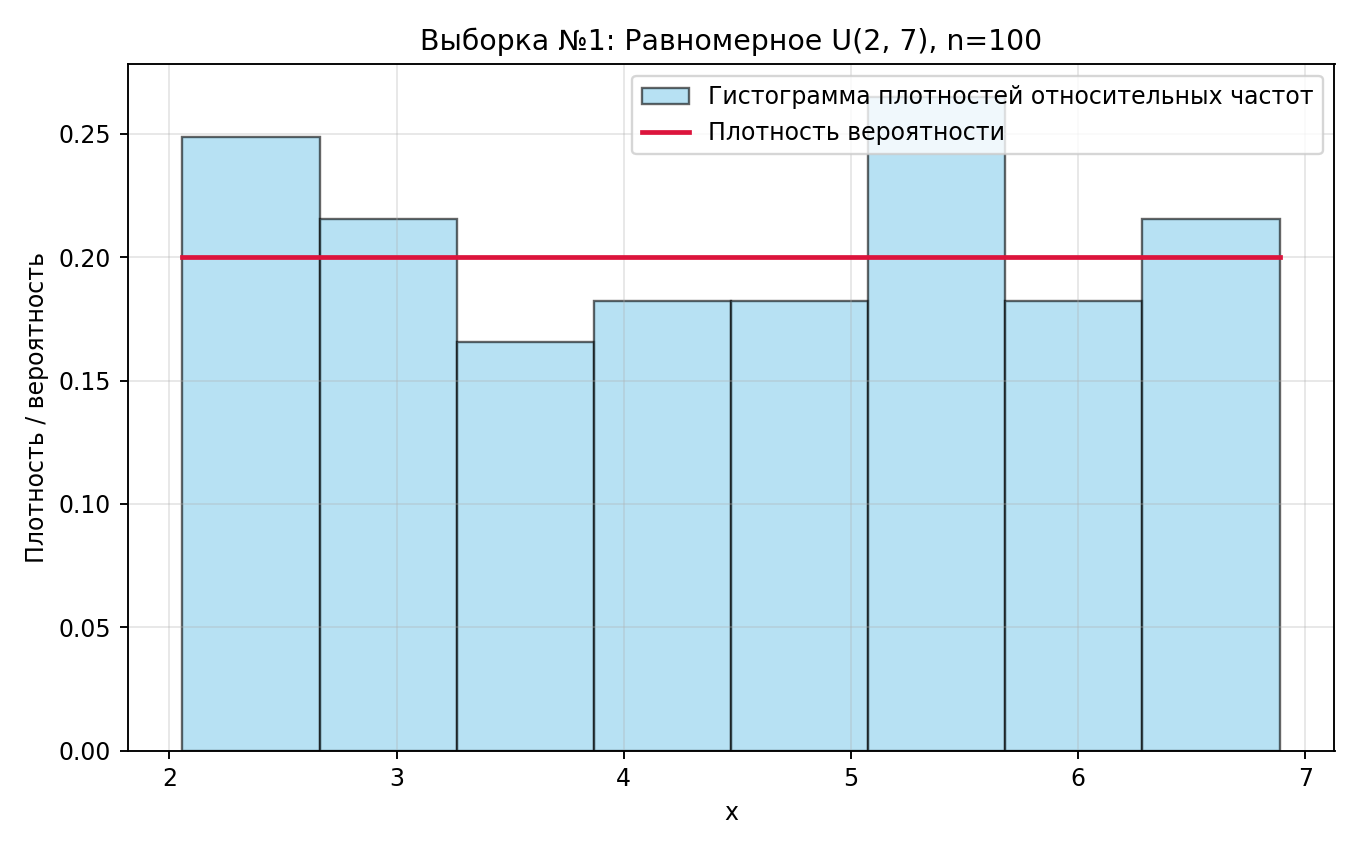
\includegraphics[width=\linewidth]{figures/sample_1.png}
        \caption{Выборка №1}
    \end{subfigure}
    \hfill
    \begin{subfigure}{0.48\textwidth}
        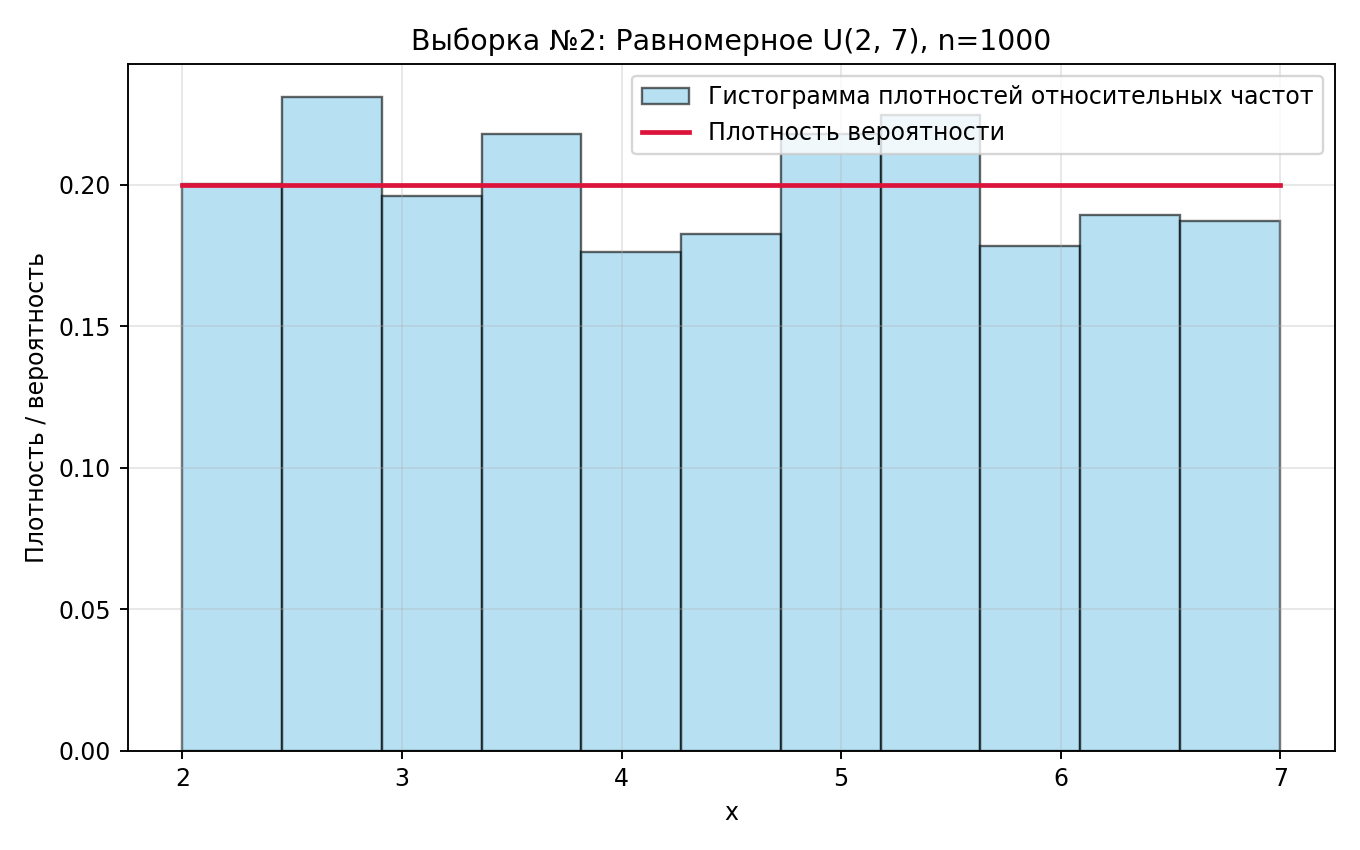
\includegraphics[width=\linewidth]{figures/sample_2.png}
        \caption{Выборка №2}
    \end{subfigure}
\end{figure}

\begin{figure}[H]
    \centering
    \begin{subfigure}{0.48\textwidth}
        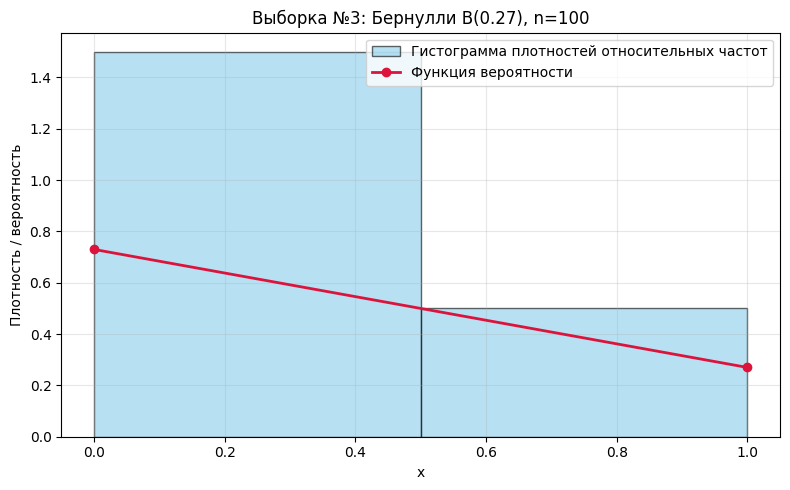
\includegraphics[width=\linewidth]{figures/sample_3.png}
        \caption{Выборка №3}
    \end{subfigure}
    \hfill
    \begin{subfigure}{0.48\textwidth}
        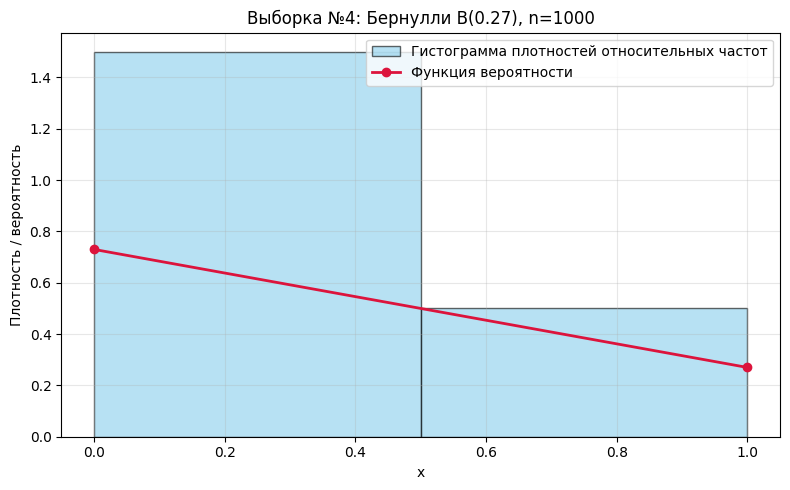
\includegraphics[width=\linewidth]{figures/sample_4.png}
        \caption{Выборка №4}
    \end{subfigure}
\end{figure}

\begin{figure}[H]
    \centering
    \begin{subfigure}{0.48\textwidth}
        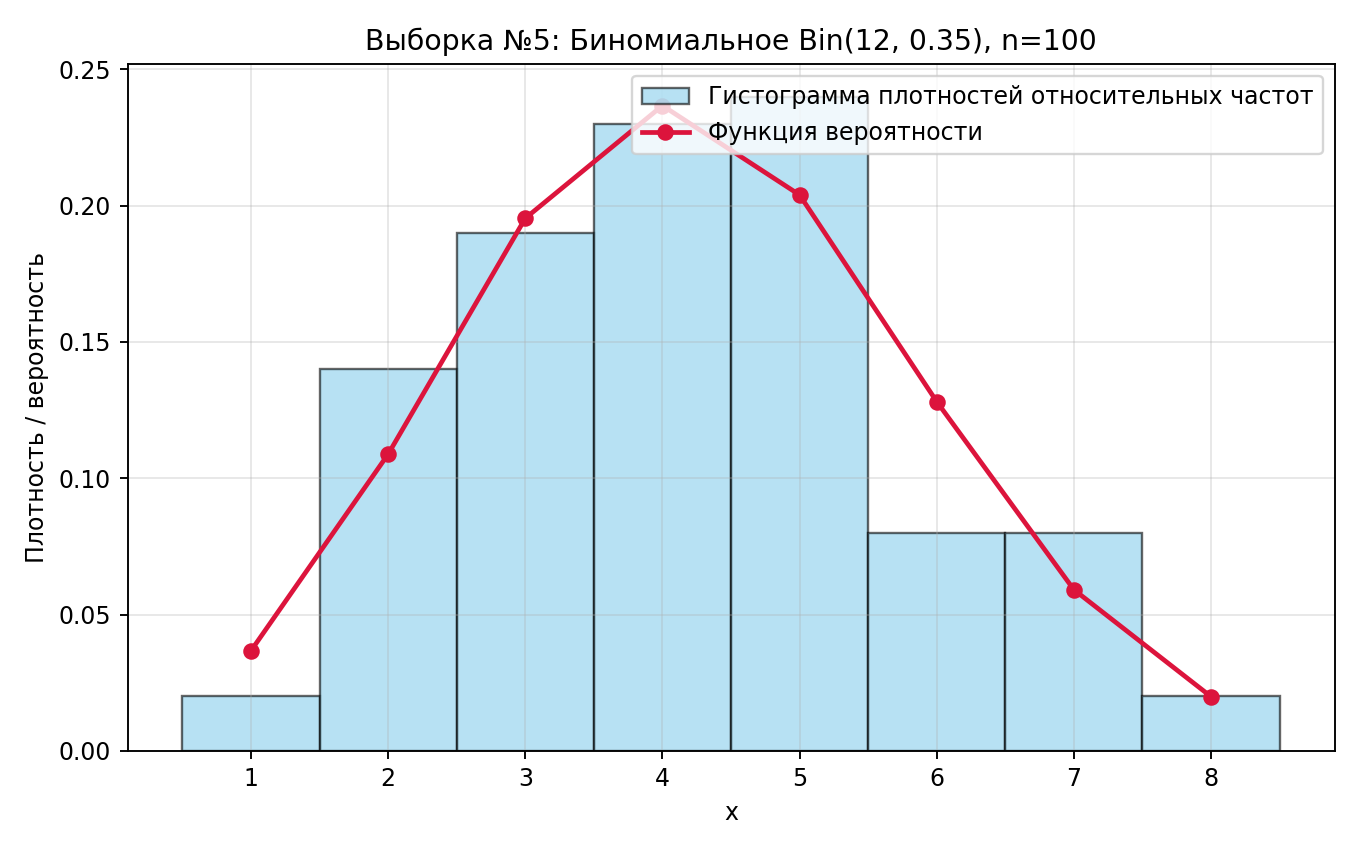
\includegraphics[width=\linewidth]{figures/sample_5.png}
        \caption{Выборка №5}
    \end{subfigure}
    \hfill
    \begin{subfigure}{0.48\textwidth}
        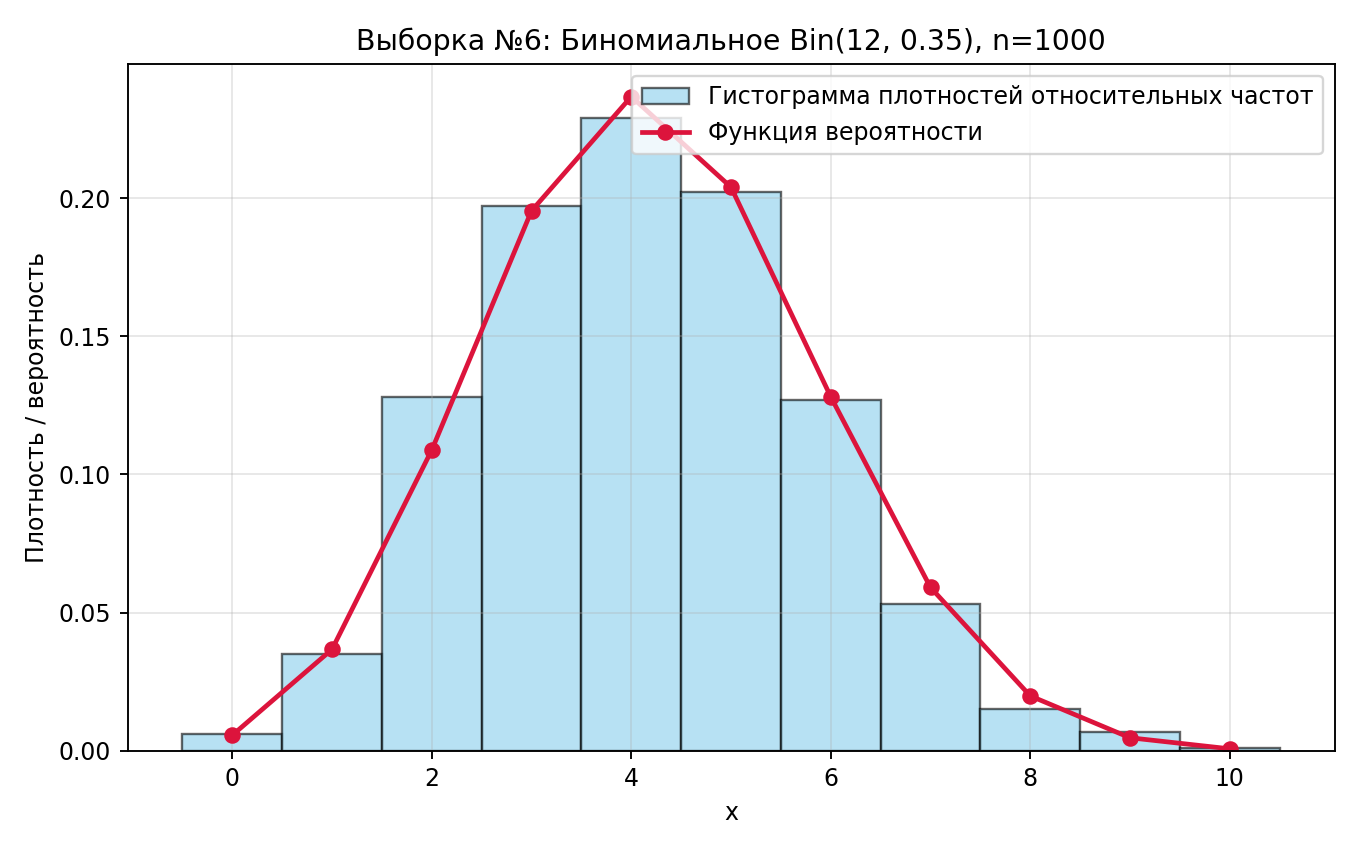
\includegraphics[width=\linewidth]{figures/sample_6.png}
        \caption{Выборка №6}
    \end{subfigure}
\end{figure}

\begin{figure}[H]
    \centering
    \begin{subfigure}{0.48\textwidth}
        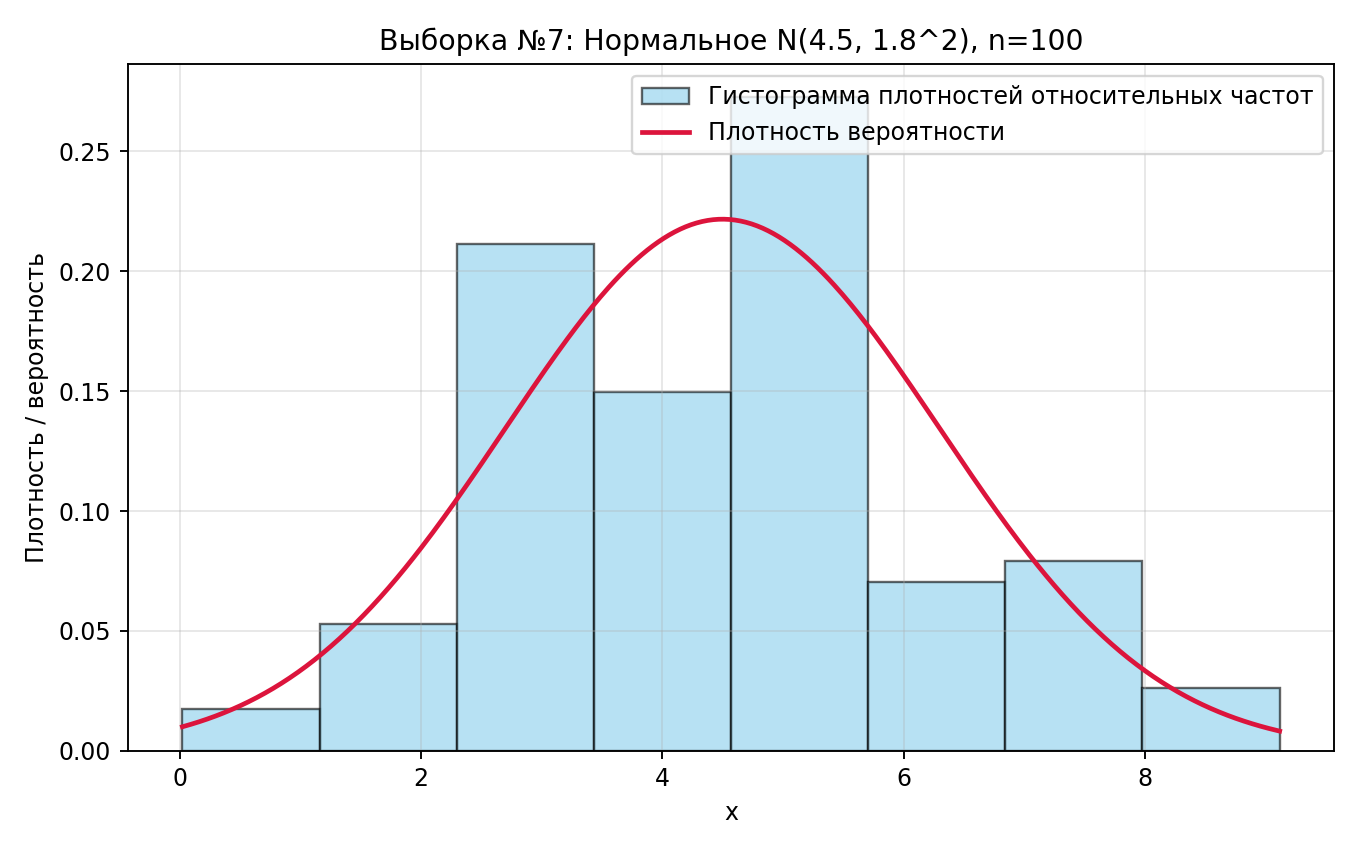
\includegraphics[width=\linewidth]{figures/sample_7.png}
        \caption{Выборка №7}
    \end{subfigure}
    \hfill
    \begin{subfigure}{0.48\textwidth}
        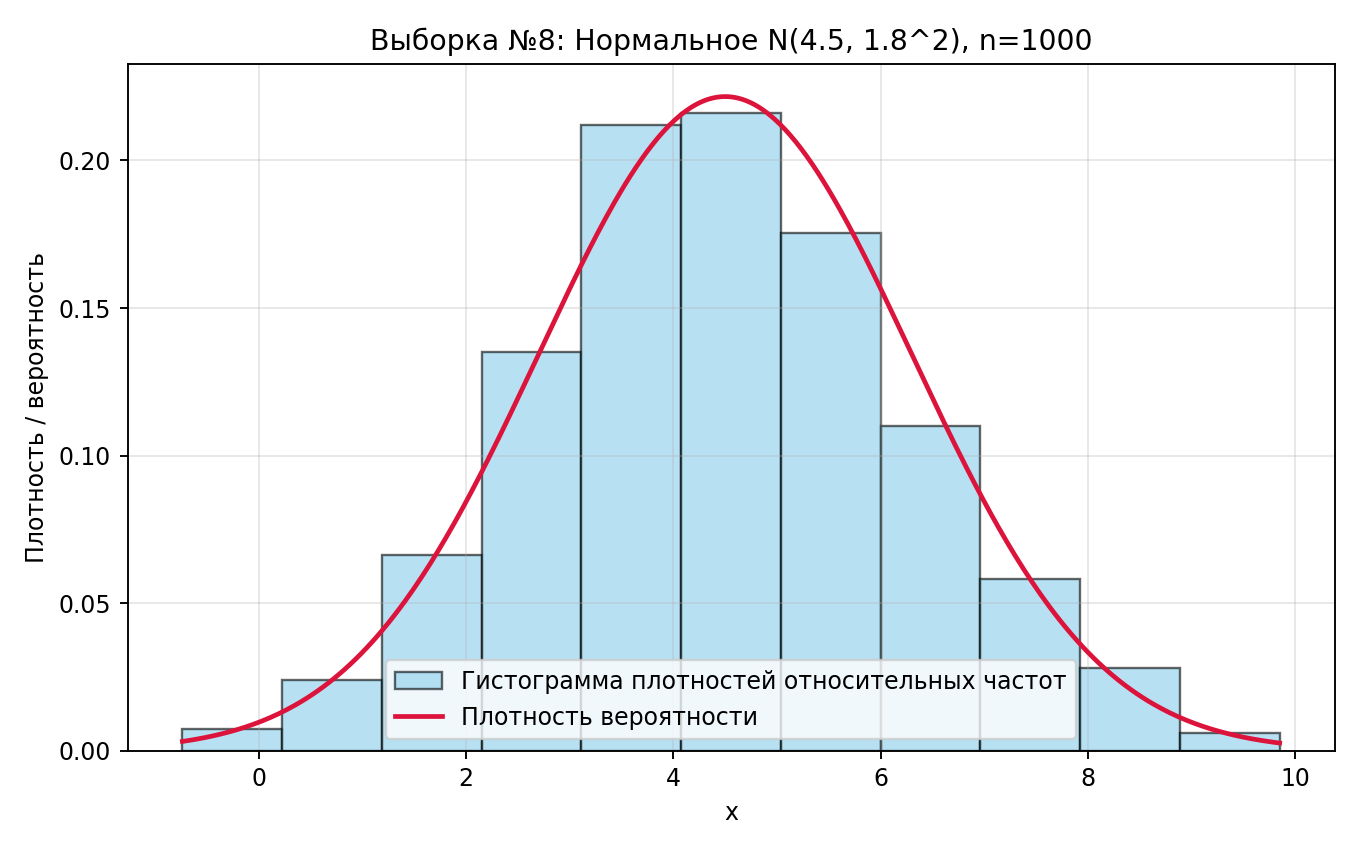
\includegraphics[width=\linewidth]{figures/sample_8.png}
        \caption{Выборка №8}
    \end{subfigure}
\end{figure}

\subsection*{3.3 Вывод в терминал}
\VerbatimInput[fontsize=\small]{results_terminal.txt}

\section*{4. Полный код программы}
\lstinputlisting[style=pycode]{lab1_full_code.py}

\end{document}
